\chapter{Tests and metrics}

After the testbed implementation, tests about its performance and metrics were
gathered in order to understand the real project effectiveness. We performed
tests relatively two main sections: one testing the architecture overall
responsivness and one checking the SFC implementation and efficiency.

\section{System responsivness}

\subsection{Docker vs Virtual Box startup measurement}

Regarding the overall system responsivness, a metric we considered worth to 
test was the VNF start up time in a docker environment versus one virtualized 
through a common virtual machine system (in this case Virtual Box was choosen). 
To make this simulation as fair as possible, we used the same node (an 
Openstack VM vith 32GB of RAM, 8 vCPU and solid state storage) and used the same 
``boot sequence'' for both the VNFs: first we launched the Astaire framework, 
ensuring its availability to process data and then we notified the test 
machine of the successful boot. The startup time was measured from the 
beginning of the startup command (\verb!docker run! for docker and 
\verb!VBoxManage -s! for Virtual Box) till the first TCP hit received by the 
test backend (to make things as smooth as possible, \verb!netcat! was used 
to listen to incoming TCP data).

It is worth saying that Docker metrics are generally more precise than the
Virtual Box one: Docker allows to inspect the container and to gain startup and
shutdown times with a precision of millseconds, while to gather this information
for VirtualBox instances we had to use the command line utility \verb!time!,
that registered timing with a precision of hundredths of a second. Nonetheless,
this didn't influence the test too much. To reduce possible outliers we perfomed
the test $100$ times. With this $N$, the total time spent by the Virtual
Machines to boot up was of $2021,15$ seconds, while with containers the same
number of start ups resulted in a total of $1.638$ seconds. Summing up, Docker
employs only the $0,08\%$ of the overall time spent for the test, underlining
how isolating the process with a set of defined policy and avoiding a
virtualized kernel boot-up saves a considerable amount of time.

\begin{figure}[H]
    \centering
    \begin{subfigure}[b]{0.4\textwidth}
        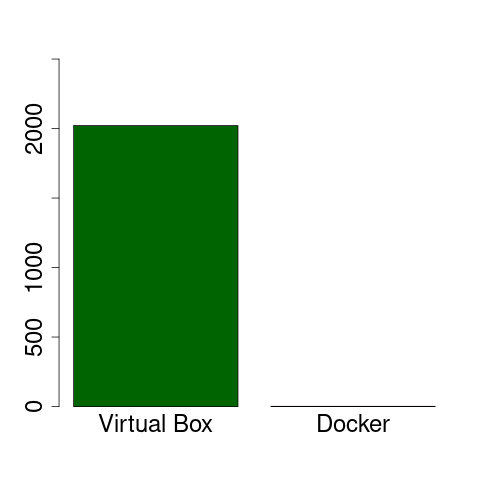
\includegraphics[scale=0.4]{docker_vs_vmBarplotGraph}
        \caption{Barplot between Virtual Box and Docker startup times in seconds
          (y-axis).}
        \label{chap:tests:sec:dockervsvb:img:barplot}
    \end{subfigure}
    ~
    \begin{subfigure}[b]{0.4\textwidth}
        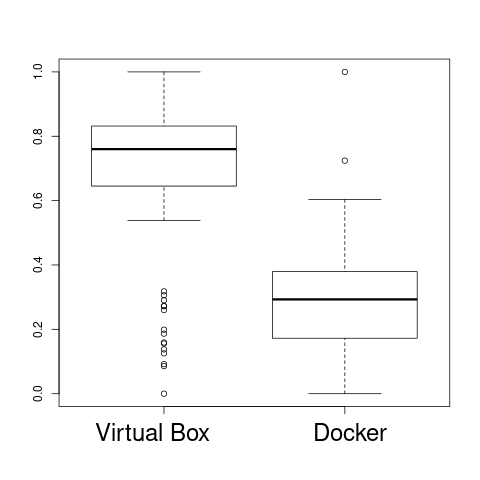
\includegraphics[scale=0.35]{docker_vs_vmBoxplotGraph}
        \caption{Boxplot between Virtual Box and Docker with values normalized 
in range $0-1$.}
        \label{chap:tests:sec:dockervsvb:img:boxplot}
    \end{subfigure}
    \caption[Virtual Box vs Docker start up comparison]{In these graphs it is
      possible to see how the total time to start up a virtual machine through
      Virtual Box is very high compared to the time required to the overall
      Docker containers to boot. A single VirtualBox instance requires on
      average 20,211 seconds to boot up, while a container requires, on average,
      only 0.016 seconds. The main reason behind this difference, as already
      explained in other parts of this thesis, it is caused by the guest's
      kernel that has to initialized itself, before starting any program. On
      Docker, instead, the kernel is the same of the host, so the only
      operations needed are to isolate the program from the rest of the OS and
      add it to the process list.}
    \label{chap:tests:sec:dockervsvb:subimg:plots}
\end{figure}


\begin{table}[t]
\centering
\resizebox{\textwidth}{!}{%
\begin{tabular}{l|c|c}
                     & \textbf{Total start up time (seconds)} & \textbf{Average start up time (seconds)} \\ \hline
\textbf{Docker}      & 1,638                                 & 0,016                                     \\
\textbf{Virtual Box} & 2021,150                              & 20,211                                 
\end{tabular}%
}
\caption[Docker vs Virtual Box start up times comparison]{Docker vs Virtual Box
  start up times comparison. Is possible to se how the overall time required to
  start $100$ containers is less than the time to start one traditional virtual
  machine. The overall time required by the traitional virtualization system is
  approximately of 33 minutes, witch gives a significant insight of how much
  time is required to create and boot a virtualized enviroment.}
\label{my-label}
\end{table}


% The overall time required by the traitional virtualization system is
% approximately of 33 minutes, witch gives a significant insight of how much time
% is required to create and boot a virtualized enviroment.


\subsection{SFC chain deploy measurement}

The previous test make us see how much Docker is faster than a traditional
virtual machine. The test, though, was performed on a single node, interacting
directly with Docker and not through the orchestrator we used in the thesis
development, Kubernetes. The following measurement will allow us to see the time
required in order to deploy an SFC of different elements in a Kubernetes
environment. The deployment consists in a Pod inside a Deployment definition
with a related Service, to simulate a real VNF. After the Pod startup, a request
is made to a backend designed to count the chain elements that have successfully
boot-up returning, eventually, the overall start up timing.

% TODO: missing YAML definition: [language=YAML]
%https://tex.stackexchan
%ge.com/questions/152829/how-can-i-highlight-yaml-code-in
%- a-pretty-way-with-listings
\lstinputlisting[caption={Kubernetes YAML configuration that has been used to
    simulate a single VNF deployment}, captionpos=b]{res/code/sfc_test.yaml}

\vspace{0.5cm}

\noindent As is possible to see from the YAML definition, the test involved, for
every launch, the VNF download from the Docker hub repositories. This, while it
forced every node to delete and download the image for each test, it ensured
consistent measurements in cases where the selected node for the deployment did
not have the image already pulled. In addition to that, another consideration
needs to be taken into account: when the chain consists of two or more elements,
the container image which is used for the container deployment is the same for
every VNF involved, thus reducing the start up time for the subsequent pods that
reside in nodes that have already deployed one.

\begin{figure}[t]
  \centering
  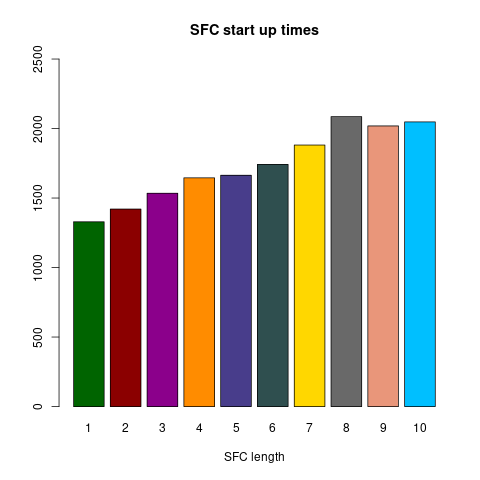
\includegraphics[scale=0.5]{sfc_startupBarplotGraph}
  \caption[SFC start-up time barplot]{SFC start-up time barplot. It is
    noticeable how there seems to be a linear correlation between the SFC
    startup time and the SFC length, even though for the chain with eight
    elements it is possible to see that the overall deploy time is more compared
    to chains with nine and ten elements.}
  \label{chap:tests:sec:sfclength:img:barplot}
\end{figure}

\begin{longtable}[c]{c|c|c}
\textbf{SFC length} & \textbf{Total deploy time (seconds)} & \textbf{Average deploy time (seconds)} \\ \hline
\endhead
%
\textbf{1}          & 1329,119                   & 13,291                       \\
\textbf{2}          & 1420,693                   & 14,207                       \\
\textbf{3}          & 1534,487                   & 15,345                       \\
\textbf{4}          & 1645,298                   & 16,453                       \\
\textbf{5}          & 1663,905                   & 16,634                       \\
\textbf{6}          & 1741,825                   & 17,418                       \\
\textbf{7}          & 1881,525                   & 18,815                       \\
\textbf{8}          & 2085,622                   & 20,856                       \\
\textbf{9}          & 2018,718                   & 20,187                       \\
\textbf{10}         & 2047,645                   & 20,476                       \\
\caption[SFC start up time]{Table of the results. It is possible to see how the
  time required for the SFC to go up increases with the length, reaching an
  average of 20 seconds for chain of eight, nine and ten elements.}
\label{chap:tests:sec:sfclength:tab:sfcdata}\\
\end{longtable}

\newpage

\paragraph*{Kubernetes specifications}
A Kubernetes installation was performed in order to carry out the test
descripted above. All the machines (master node and minions) involved had the
same specifications i.e., 4GB of RAM, 2 vCPU and 10GB of SSD storage.
Nonetheless the constrained resources, absolutely far from a real Kubernetes
production environment, is possible to notice how, even with a chain of ten
elements, the average time required to deploy an SFC is equal, if not smaller,
of the time required to deploy a Virtual Box machine on an instance with 32GB of
RAM, 8 vCPU and 50GB of SSD storage.
% graphs, talk about them

\section{Final considerations}

In these tests is possible to see one critical aspect concerning an architecture
that follows the containerization approach: great flexibility in terms of
deployments. This possibility to deploy services in the form of SFCs and VNFs in
a very small amount of time is one of the key point required in the new 5G
architecture, that the tests above demonstrated this project is able to adhere.
Finally, the ability to rapidly redeploy software means smooth and easier
software development lifecycle, where developers have the possibility to
automatically push ``fresh'' software in production, letting the MANO and thus
the container orchestrator handling all the difficult and delicate tasks to put
software in a production environment, eliminating the possibility of human
errors and assuring longer uptimes.
